\subsection{Coulomb friction}
The objective of this activity is display the UR5 robot on rviz and control the motion of its joints with inverse dynamics control method with compliant contact. The simulation starts with the initial joint position $\begin{bmatrix} \pi & -\frac{\pi}{8} & -\frac{\pi}{6} & 0.0 & 0.0 & 0.0 \end{bmatrix}$ rad, joint velocity $\begin{bmatrix} 0.0 & 0.4\pi & 0.0 & 0.0 & 1.2\pi & 0.0 \end{bmatrix}$ and external force $\begin{bmatrix} 0.0 & 0.0 & 0.0 \end{bmatrix}$ N. The second and fifth joints will move following a sinusoidal trajectory during the first 4 seconds and maintain a constant joint position during the last second. Finally, in this activity, the sinusoidal trajectory will be modified from $4$ seconds to $5$ seconds.

Figure \ref{fig:act_2.8_mu_0.2_joint_position} and \ref{fig:act_2.8_mu_0.8_joint_position} show the trajectory tracking of all joints of UR5 robot with $\mu=0.2$ and $\mu=0.8$.

\begin{lstlisting}[language=Python,caption={Move the second and fifth joint of UR5 robot with the required movement of activity 2.8.}, label={lst:inverse_dynamics_coulomb_friction}]
# =========================
#   Configuration of node
# =========================
# create a node: 
rospy.init_node("node_inverse_dynamics_coulomb_friction")

# public in topic /joint_states	to send joint data	
pub = rospy.Publisher('joint_states', JointState, queue_size=1000)

# loop rate (in Hz)
rate 	= rospy.Rate(1000)		# 100 [Hz]
dt 		= 1e-3					# 10  [ms]

# object(message) type JointState
jstate = JointState()

# ==========================================
#   Set initial joint configuration of UR5
# ==========================================
# initial configuration: position, velocity and acceleration 
q0 =   np.array([np.pi, -np.pi/8,  -np.pi/6, 0.0, 0.0, 0.0])
dq0 =  np.array([0.0, 0.4*np.pi, 0.0, 0.0, 1.2*np.pi, 0.0]) 
ddq0 = np.array([0.0, 0.0, 0.0, 0.0, 0.0, 0.0]) 

# desired trajectory: position, velocity and acceleration
q_des =   np.array([np.pi, -np.pi/8,  -np.pi/6, 0.0, 0.0, 0.0]) 
dq_des =  np.array([0.0, 0.0, 0.0, 0.0, 0.0, 0.0]) 
ddq_des = np.array([0.0, 0.0, 0.0, 0.0, 0.0, 0.0]) 

# measured trajectory: position, velocity and acceleration
q =   np.array([np.pi, -np.pi/8,  -np.pi/6, 0.0, 0.0, 0.0])
dq =  np.array([0.0, 0.4*np.pi, 0.0, 0.0, 1.2*np.pi, 0.0]) 
ddq = np.array([0.0, 0.0, 0.0, 0.0, 0.0, 0.0]) 

# ===========================
#   UR5 robot configuration
# ===========================
# joints name of UR5 robot
jnames = ['shoulder_pan_joint', 'shoulder_lift_joint', 'elbow_joint','wrist_1_joint', 'wrist_2_joint', 'wrist_3_joint']

# number of degress of freedom
ndof = 6
# the class robot load the ur5.urdf
ur5_robot = Robot(ndof,q0, dq0, dt)
# create inertia matrix 
M = np.zeros([ndof,ndof])
# create nonlinear effects vector
b = np.zeros(ndof)

# ===============================
#   PD controller configuration
# ===============================
# proportional gain
kp = 600*np.ones(ndof)
# derivative gain
kd = 2*np.sqrt(kp[0])*np.ones(ndof)
# control vector
tau = np.zeros(ndof) 

# =============================
#   Enviornment configuration
# =============================
p0 = np.array([0.0, 0.0, 0.0]) # m
k_env = 10000*np.ones(3) # N/m
d_env = 1000*np.ones(3) # N.s/m
n = np.array([0, 0, 1])
mu = 0.2
#===============
#   Simulation
#===============
t = 0.0             # [sec] 
sim_duration = 5.0  # [sec]
sine_duration = 5.0 # [sec]
force_start   = 1.0 # [sec]


while not rospy.is_shutdown():
    # generate sinusoidal joint reference
    if t<=sine_duration:
        # second link
        q_des[1], dq_des[1], ddq_des[1] = sinusoidal_reference_generator(q0[1], 0.2, 1, t)
        last_q_des_1 = q_des[1]
        # fifth link
        q_des[4], dq_des[4], ddq_des[4] = sinusoidal_reference_generator(q0[4], 0.4, 1.5, t)  
        last_q_des_4 = q_des[4]  
    else:
        # second link
        q_des[1], dq_des[1], ddq_des[1] = step_reference_generator(0, last_q_des_1)
        # fifth link
        q_des[4], dq_des[4], ddq_des[4] = step_reference_generator(0 , last_q_des_4)

    # position of end-effector
    p_ee = fkine_ur5(q)[0:3,3]
    # position jacobian
    J = jacobian_xyz_ur5(q)    
    # velocity of end-effector
    dp_ee = np.dot(J, dq)

    if (np.dot(n, p0-p_ee))<0:
        # external force
        f_ext = np.multiply(k_env, p0-p_ee) - np.multiply(d_env, dp_ee) # N
        if f_ext[0]>= mu*f_ext[2]:
            f_ext[0] = mu*f_ext[2]
        if f_ext[0]<= -mu*f_ext[2]:
            f_ext[0] = -mu*f_ext[2] 

        if f_ext[1]>= mu*f_ext[2]:
            f_ext[1] = mu*f_ext[2]
        if f_ext[1]<= -mu*f_ext[2]:
            f_ext[1] = -mu*f_ext[2] 
        # external torque 
        tau_ext = np.dot (J.transpose(), f_ext) # N.m
    else:
        # external torque 
        tau_ext = np.zeros(6) # N.m
    print("f_ext: ", f_ext)
    # error: position and velocity
    e 	=  q_des - q
    de 	=  dq_des - dq    

    # compute inertia matrix
    M = ur5_robot.get_M()

    # compute nonlinear effects vector
    b = ur5_robot.get_b()   

    # control law: PD control + Feedback linearization
    tau = M.dot(ddq_des +  np.multiply(kp, e) + np.multiply(kd, de)) + b + tau_ext
    
    # send control signal   
    ur5_robot.send_control_command(tau)
    # update states
    q, dq, ddq = ur5_robot.read_joint_position_velocity_acceleration()

    # publish message
    jstate.header.stamp = rospy.Time.now()
    jstate.name 		= jnames			# Joints position name
    jstate.position 	= q
    jstate.velocity 	= dq
    pub.publish(jstate)

    # update time
    t = t + dt

    # stop simulation
    if t>=sim_duration:
        print("stopping rviz ...")
        break
    rate.sleep()
\end{lstlisting}

\begin{figure}[H]
    \centering
    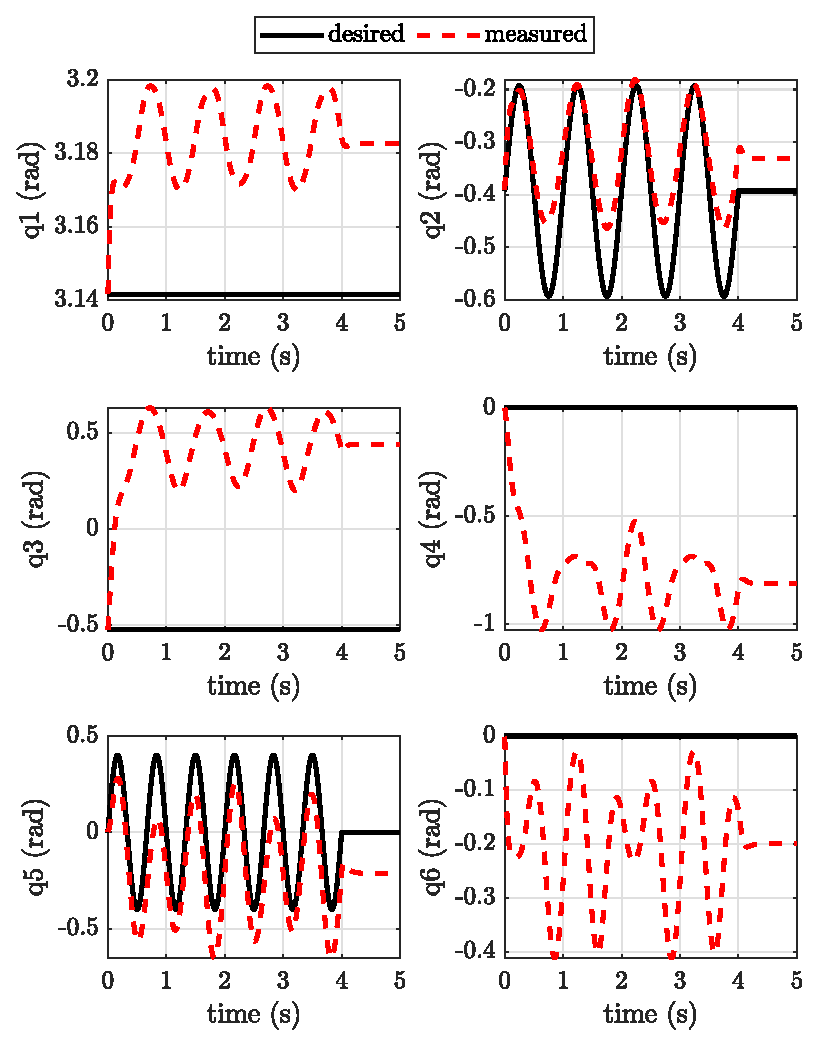
\includegraphics{images/act_2.8_mu_0.2/joint_position.eps}
    \caption{Angular position of each joint of UR5 robot with Algorithm \ref{lst:inverse_dynamics_coulomb_friction}}
    \label{fig:act_2.8_mu_0.2_joint_position}
\end{figure}

\begin{figure}[H]
    \centering
    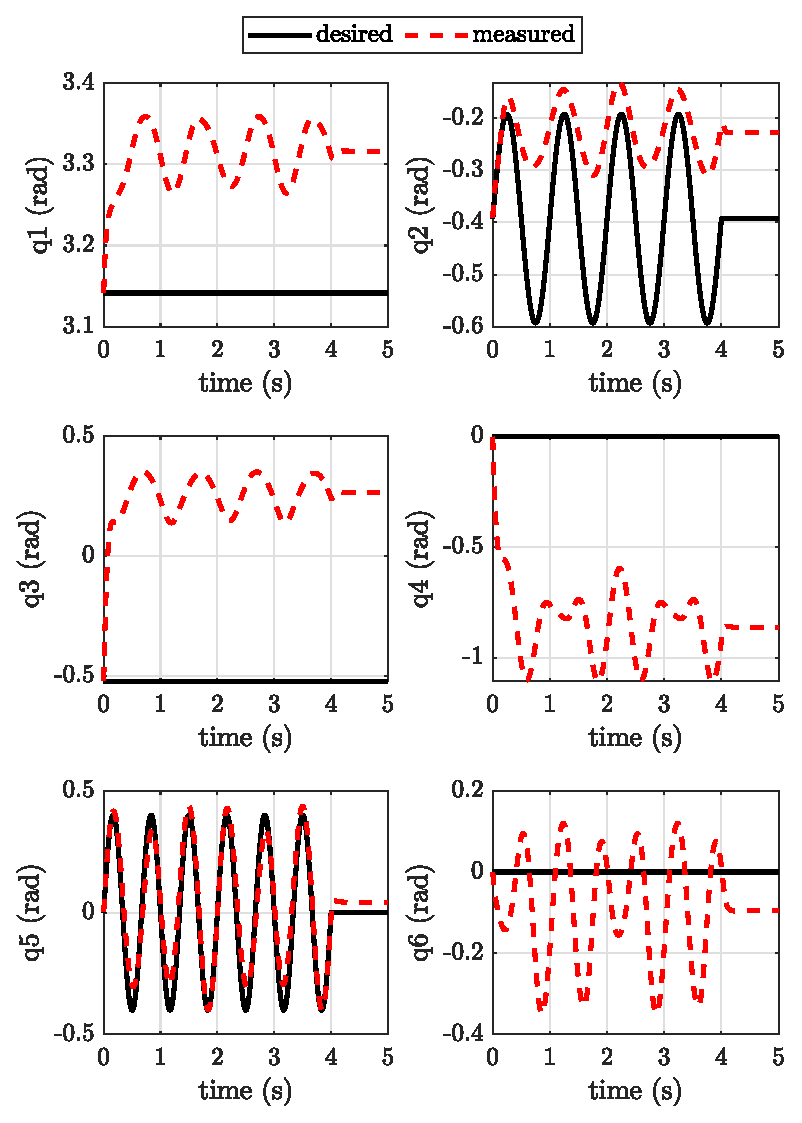
\includegraphics{images/act_2.8_mu_0.8/joint_position.eps}
    \caption{Angular position of each joint of UR5 robot with Algorithm \ref{lst:inverse_dynamics_coulomb_friction}}
    \label{fig:act_2.8_mu_0.8_joint_position}
\end{figure}
